% !TEX program = pdflatex
\documentclass[preprint,10.5pt]{article}

\usepackage{listings}
\usepackage{tasks}
\usepackage{graphicx}
\usepackage{hyperref}
\usepackage{graphicx}
\graphicspath{{images/}}
\pagenumbering{gobble}

\usepackage[                                                                       
 paper  = letterpaper,                                                            
 left   = 1.0in,                                                                 
 right  = 1.0in,                                                                 
 top    = 0.5in,                                                                  
 bottom = 0.5in,                                                                  
 ]{geometry}

\hypersetup{
    colorlinks=true,
    linkcolor=blue,
    filecolor=magenta,      
    urlcolor=purple,
}

\begin{document}

\title{Deep Learning $|$ Final Project Proposal}
\author{Michael Alvarino (maa2282), Richard Dewey (rld2126), Colby Wise (cjw2165)}

\maketitle

\section{Proposal}
\paragraph{One-liner} We intend to build a network to predict user ratings of movies based on a user's other categorical data, ratings of the movie in question, and importantly, the text document of their review. Our model will be based on Google's \href{https://arxiv.org/pdf/1606.07792.pdf}{Wide and Deep Learning}, which was originally designed to handle sparse matrices of categorical data, but expand upon it to include text.

\paragraph{The Problem} Prior to deep learning, standard approaches for recommendation systems ($RecSys$) used collaborative filtering which relies on decomposing users, items (i.e. movies), and ratings into latent feature matrices. Then the weights of these matrices are used to predict a rating a user would give for an item. However, collaborative filtering handles sparse data poorly. To alleviate the sparsity problem, Google created Wide and Deep networks. Unfortunately, Wide and Deep networks were built to handle simple, categorical features alone. Our model will expand upon Wide and Deep to include text data, specifically movie reviews, within the deep portion of the network.
\par We will do this by stacking a recurrent neural network on top of the deep portion in order to generate an embedding for the reviews created by users (see diagram below). By including such rich data into our model, we expect to see better generalization and more accurate prediction of movie ratings. For a more detailed diagram of the model, see our diagrams section.
\par Our first step will be to re-implement the Wide and Deep network using our dataset rather than the toy dataset used in the example online. By the November 23 milestone, we expect to have completed the standard Wide and Deep implementation, and be ready to implement the recurrent neural network portion of our model.

\paragraph{Data} We intend to use one primary dataset, Amazon Instant Video ($AIV$). The complete dataset consists of 7,911,684 reviews of the following columns: productId, userId, profileName, helpfulness, score, time, summary, and text. If handling and training on such a large dataset becomes an issue, we intend to use either a random subset (of about 40,000 dat points) we generate ourselves, or one of those random subsets that already exists online.

\paragraph{Previous Work and References} The literature on recommendation systems is deep, but because we will be focusing on expanding the Wide and Deep approach, our primary reference will be the original \href{https://www.tensorflow.org/tutorials/wide_and_deep}{Wide and Deep} paper. For this particular paper there are multiple learning resources available online, from \href{https://www.tensorflow.org/tutorials/wide_and_deep}{tutorials}, to \href{https://github.com/tensorflow/tensorflow/blob/master/tensorflow/examples/learn/wide_n_deep_tutorial.py}{source code}, to \href{https://www.youtube.com/watch?v=NV1tkZ9Lq48}{videos}.
\par Our expansion on the method will create an embedding of a large document, similar to the encoder portion described in the \href{https://web.stanford.edu/class/cs224n/reports/2746634.pdf}{News Article Summarization} paper. For this paper the exact source code is not available, however there are many \href{https://github.com/hengluchang/deep-news-summarization}{open-source examples}. Importantly, we will only be using the encoding half of of the News Article Summarization work.

\paragraph{Evaluation Criteria} Since the output of our model will be an integer score out of 5 for a movie (higher being better), we intend to evaluate with standard point value error estimates, specifically cross entropy loss. Our true measure of success will be the comparison of our model (including text data embeddings) against a standard Wide and Deep model (using only categorical data). We expect to see improved generality and more accurate rating scores.

\paragraph{Further Research} An important part of Google's Wide and Deep model is the efficiency of the network. By adding recurrent neural networks to process text data, we are significantly increasing the network complexity. It would be interesting to analyze that complexity and the time required for a single rating prediction to determine if our network is practical for a production environment.

\section{Diagrams}
\paragraph{Final Model Diagram} \ \newline
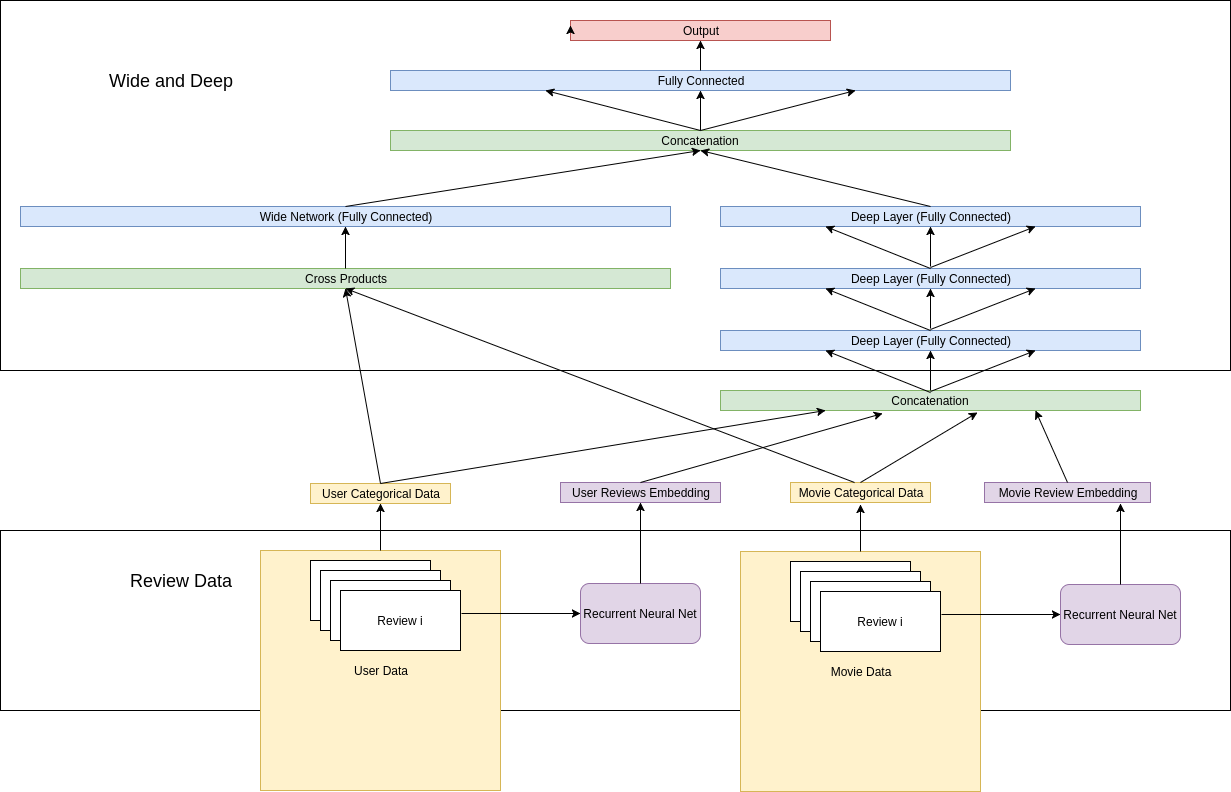
\includegraphics[scale=0.38]{network_diagram}

\end{document}